\documentclass[12pt,fleqn]{article}\usepackage{../../common}
\begin{document}
Felzenswalb Gruplaması (Felzenswalb Clustering)

Minimum Kapsayan Ağaç (Minimum Spanning Tree -MST-) kavramını kullanan
Felzenswalb kümelemesini göreceğiz. MST'yi daha önce işledik. Literatürde
Felzenswalb metotunun imaj gruplaması için kullanıldığı görülebilir, biz
imaj gruplaması yapan algoritma içinden veri kümelemesi yapan kısmı
çıkarttık ve ayrı bir şekilde paylaşıyoruz. Bu gruplama algoritmasının daha
önce paylaştığımız Kruskal'ın MST koduna yapılacak birkaç ekleme sayesinde
elde edilebilmesi hakikaten ilginç. Normal MST çizitin ayrı bölgelerinde
ayrı ağaçlar yaratır ve bunları yavaş yavaş büyütür, gerektiği noktalarda
onları birleştirir. Felzenswalb sadece bu birleştirme mantığını biraz
değiştirip, ayrı ağaçları bir grup olarak kabul eder, ve bu grupların kendi
içinde benzerliği maksimal, gruplararası benzerliği minimal olacak hale
getirir. Bu şekilde bildik Kruskal işletilince çok hızlı işleyen hızlı bir
gruplama algoritması elde edilmiş olur!

Felzenswalb veri olarak, MST gibi, bir çizit alır ve bu çizit veri
noktalarının arasındaki yakınlık bilgisini içeren bir matris olarak
verilebilir. Mesela 5 veri noktası var ise, 0. nokta ile 1. nokta
arasındaki '10' büyüklüğündeki bir mesafe $A(0,1) = 10$ olarak
kaydedilebilir. Kümeler birbirine yakın öğeler arasından seçilir.

Algoritmanın önemli avantajlarından biri küme sayısının (GMM'de olduğu
gibi) önceden tanımlanmasına gerek olmamasıdır. Belli eşik değerleri
tanımlanınca küme sayısı kendiliğinden bulunur. Tabii ``dışarıdan verilen
bir parametreyi başka biriyle değiştirmiş mi olduk?'' sorusu akla
gelebilir, Felzenswalb'ın aldığı hiperparametreler kabaca ayarlanabilen ve
veri kaynağı bağlamında akla uygun şeyler, ve belli değerler etrafında
stabilite ortaya çıkabiliyor. Kıyasla ``küme sayısı'' ciddi bir rakam ve
değişmesi mümkün değil. 

Felzenswalb'ın matematiğinde önce imaj bölgelerinin (ya da veri kümeleri
olarak düşünebiliriz) arasında ikili karşılaştırma için bir ölçüt
gerekir. Bu bölümde bir beyan $D$'yi ortaya koyacağız, ki bu beyan,
imajdaki iki bileşen (ki imaj gruplamasının doğru olarak bulmaya çalışacağı
bileşenler) arasında bir sınır olup olmadığına dair kanıtın ölçüsü
olacak. Beyanın temeli şudur: iki bileşen arasındaki sınırın boyunda yer
alan her iki tarafın öğelerinin farklılığına bak, ve onu her bileşenin
kendi içindeki farklılığa göre oranla. Yani bu beyan, bir bileşenin iç
farklılığını dış farklılığına kıyaslar, ve bu sebeple verinin yerel
karakteristikleri gözetmiş olur. Kıyaslama mesela, global, verinin her
yerinde aynen geçerli olacak bir sabit eşik değerine vs. bağlı değildir.

Tanım

Bir bileşen $C \subseteq V$, ki $C$ bir bileşendir (component) ve $V$ çizitin tüm
noktalarıdır, {\em iç farklılığını}, o $C$'nin minimum kapsayan ağacının,
yani $MST(C)$'sinin en büyük kenar ağırlığı olarak alıyoruz. Bu iç farklılığı
$Int(C)$ olarak belirtirsek, 

$$ Int(C) = \max_{e \in MST(C,E)} w(e) $$

ki $w((v_i , v_j))$ bir çizit $G = (V,E)$'yi oluşturan bir kenar $(v_i,v_j)
\in E$ ağırlığı olarak belirtilir. 

Tanım

İki bileşen $C_1,C_2 \subseteq V$ arasındaki farkı o iki bileşeni
birleştiren kenarlardan en ufağı olarak alıyoruz. İki bileşenin arasında
birden fazla bağlantı olması mümkündür, tüm bunlara bakıyoruz, ve en
ufağını alıyoruz.

$$ Dif(C_1,C_2) = \min_{v_i \in C_1, v_j \in C_2, (v_i,v_j) \in E} w((v_i,v_j))$$

Eğer $C_1,C_2$ arasında bir kenar yok ise $Dif(C_1,C_2) = \infty$ kabul
ediliyor. 

Prensip olarak iki bileşen arasındaki en minimal bağlantının problem
çıkartabileceği düşünülebilirdi, niye en az, niye ortalama vs değil?  Pratikte
bu ölçütün çok iyi işlediği görülmüştür. Hatta iyi olmaktan öte, bu ölçüt
minimal yerine medyan, ya da diğer yüzdelik dilim (quantile) ölçütle
değiştirildiği zaman (ki bunu yaparak genel algoritmanın aykırı değerlere
-outlier- karşı daha dayanıklı olması istenmişti), algoritma çetrefilliği NP-Zor
haline geliyor. Yani gruplama kriterinde ufacık bir değişiklik problemin çözüm
zorluluğunda müthiş bir değişim ortaya çıkartıyor.

Şimdi iki bileşenin karşılaştırma beyanı $D$'nin tanımına geldik. $D$ ölçütü,
$Dif(C_1,C_2)$'nin $Int(C_1)$ ya da $Int(C_2)$'den herhangi birinden daha büyük
olup olmadığına bakar. Ayrıca bu karşılaştırmayı bir eşik değeri üzerinden pay
ekleyerek yapar, eğer irdeleme olumlu ise, iki bileşen arasında sınır vardır,
yoksa yoktur.

$$ 
D(C_1,C_2) = 
\left\{ \begin{array}{ll}
\textrm{Doğru} & \textrm{ Eğer } Dif(C_1,C_2) > MInt(C_1,C_2) \textrm{ ise } \\
\textrm{Yanlış} & \textrm{ Diğer durumda }
\end{array} \right.
 $$

Minimum iç fark $MInt$ ise şöyle tanımlıdır,

$$ 
MInt(C_1,C_2) = \min (Int(C_1)+\tau(C_1), Int(C_2)+\tau(C_2))
 $$

Eşik fonksiyonu $\tau$ üstteki irdelediğimiz fark hesaplarının belli
derecelerde dışarıdan etkilemek için koyulmuştur. Eğer bu kullanılmasaydı
sadece $Int$ fonksiyonu kullanılması gerekecekti, fakat bu ölçüt tek
başına ufak bir bileşenin yerel karakteristiklerini göstermesi açısından yeterli
değildir. Aşırı durumda mesela $|C| = 1,Int(C)=0$, yani en küçük $C$
durumudur bu ($|C|$ bileşenin içindeki öğe sayısı), içinde tek öğe vardır,
ve hiçbir kenar yoktur, $Int(C) = 0$.  

Bu sebeple iyi bir $\tau$ bileşenin büyüklüğünü hesaba katarak, ona ters
oranlı bir rakam oluşturursa iyi olur, mesela bir sabit $k$ üzerinden,

$$ \tau(C) = \frac{k}{|C|} $$

Bu demektir ki ufak bileşenler için daha kuvvetli bir ispat arıyoruz, çünkü
küçük $|C|$, $\tau$'yu büyütecektir, ve $Dif$'in ondan büyük olması daha
zorlaşacaktır. Tabii dikkat edelim, $k$ bir ``bileşen sayısı'' değildir,
yani fonksiyona dikkatli bakarsak, eğer bileşenler arasında yeterince büyük
bir fark var ise ufak bileşenlere hala izin verilmiştir.

Algoritma şöyledir, girdi olarak $G=(V,E)$ alır, ve $V$'yi $S$
bileşenlerine ayırır ki her $S$ içinde ona ait olan kenarlar vardır, yani
$S=(C_1,..,C_r)$ 

\verb!felzenswalb!$\left(G\right)$
\begin{enumerate}
  \item $E$ kenarlarını $\pi = (o_1,..,o_m)$ şeklinde küçükten büyüğe doğru
    sırala.
  \item İlk başta $S^0$ gruplamasını al. Bu durumda her kenar $v_i$
    kendi bileşeni içindedir.
  \item Her $q = 1,..,m$ icin
  \begin{itemize}
  \item $S^{q-1}$ gruplamasını baz alıp $S^q$ gruplamasını şöyle yarat;
    $q$'inci sıradaki kenarın birleştirdiği noktaların $v_i,v_j$ olduğunu
    farz edelim, yani $o_q = (v_i,v_j)$.
  \item Eğer $v_i,v_j$ $S^{q-1}$ gruplaması içinde farklı iki bileşen
    içindeyseler, ve $w(o_q)$ her iki bileşenin içsel farkına kıyasla çok
    küçük ise, bu iki bileşeni birleştir, yoksa hiçbir şey yapma.
  \end{itemize}
  \item \verb!return! $S^m$ 
\end{enumerate}

Üstteki döngü içindeki en son irdelemede içsel farktan bahsediliyor, bu
tabii ki $MInt(C_1,C_2)$. Daha formel şekilde $MInt(C_1^{q-1},C_2^{q-1})$
çünkü bileşenlerin içerikleri hangi adımda olduğumuza göre değişebilir, $q$
adımında bir önceki $q-1$'den bize ``miras kalan'' gruplamalar ve
bileşenler üzerinden iş yapıyoruz. Bir sonraki adıma ya birleşmiş, ya da
birleşmemiş (aynı) gruplamaları aktarıyoruz. 

Aynı algoritmanın biraz daha fazla formül içeren hali [3]

\verb!felzenswalb!$\left(G\right)$
\begin{enumerate}
  \item Bütün kenarları küçükten büyüğe doğru sırala.
  \item İlk başta kenar $v_i$ kendi bileşeni içinde olsun, buna $S^0$ gruplaması diyelim.
  \item Her tüm kenarlar $e_i = (v_1,v_2) \in E$ için
    \begin{itemize}
    \item $v_1 \in C_1$ ve $v_2 \in C_2$'nin birbirinden ayrı, ayrı
      bileşenler içinde ama aynı kenarı içeren noktalar olduğunu düşünelim,
    \item \verb!if! $w(e_i) \le MInt(C_1,C_2)$ ise, o zaman
    \item  $C_1$ ve $C_2$'yi birleştir
    \item \verb!else!
    \item $S^i = S^{i-1}$ 
   \end{itemize}
   \verb!return!
\end{enumerate}

Felzenswalb gruplamasının Python ile yazılmış örneği alttadır, daha hızlı
işleyen C++ bazlı kodu şurada [2] bulunabilir.

\inputminted[fontsize=\footnotesize]{python}{felz.py}

Basit bir örnek

\begin{minted}[fontsize=\footnotesize]{python}
import scipy.sparse as sps, felz
import scipy.io as io
X = io.mmread('simple.mtx')
clf = felz.Felzenswalb(min_size=1,c=1.0)
clf.fit(X)
print clf.labels_    
\end{minted}

\begin{verbatim}
(5, 5)
[1, 1, 3, 3, 1]
\end{verbatim}

Biraz daha çetrefil bir örnek

\begin{minted}[fontsize=\footnotesize]{python}
import scipy.sparse as sps
import scipy.io as io, random
import pandas as pd, os, sys
syn = pd.read_csv("../kmeans/synthetic.txt",comment='#',names=['a','b'],sep="   ")
data = np.array(syn)

from sklearn.metrics.pairwise import euclidean_distances
X = euclidean_distances(data, data)

X2 = X.copy()
# filter out large values / distances so matrix can be sparse
X2[X > 2000] = 0.0
X3 = sps.lil_matrix(X2)
X4 = sps.triu(X3)
print 'non-zero items', len(X4.nonzero()[0])
print X4.shape
\end{minted}

\begin{verbatim}
non-zero items 87010
(3000, 3000)
\end{verbatim}

\begin{minted}[fontsize=\footnotesize]{python}
import felz
clf = felz.Felzenswalb(min_size=20,c=800)
clf.fit(X4)
\end{minted}

\begin{verbatim}
(3000, 3000)
\end{verbatim}

\begin{minted}[fontsize=\footnotesize]{python}
syn['cluster'] = clf.labels_
print len(syn['cluster'].unique()), 'clusters found'
print syn[:5]
\end{minted}

\begin{verbatim}
19 clusters found
       a      b  cluster
0  54620  43523      120
1  52694  42750      120
2  53253  43024      120
3  54925  42624      120
4  54973  43980      120
\end{verbatim}

\begin{minted}[fontsize=\footnotesize]{python}
import random
for clust in syn['cluster'].unique():
    tmp = np.array(syn[syn['cluster'] == clust][['a','b']])
    plt.scatter(tmp[:,0], tmp[:,1], c=np.random.rand(3,1))
plt.savefig('mstseg_01.png')
\end{minted}

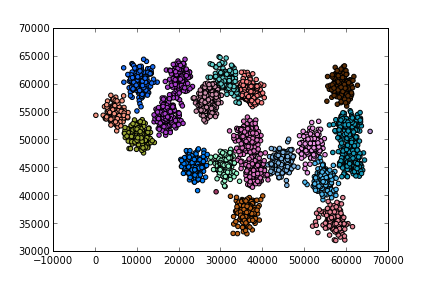
\includegraphics[height=6cm]{mstseg_01.png}

Şimdi [4] yazısında gördüğümüz kelime gruplaması örneğini Felzenswalb ile
gruplayalım.

\begin{minted}[fontsize=\footnotesize]{python}
import scipy.linalg as lin
import scipy.sparse as sps
import itertools, sys
sys.path.append('../svdcluster/')
import leven

words = np.array(
    ['the', 'be', 'to', 'of', 'and', 'a', 'in', 'that', 'have',
     'I', 'it', 'for', 'not', 'on', 'with', 'he', 'as', 'you',
     'do', 'at', 'this', 'but', 'his', 'by', 'from', 'they', 'we',
     'say', 'her', 'she', 'or', 'an', 'will', 'my', 'one', 'all',
     'would', 'there', 'their', 'what', 'so', 'up', 'out', 'if',
     'about', 'who', 'get', 'which', 'go', 'me', 'when', 'make',
     'can', 'like', 'time', 'no', 'just', 'him', 'know', 'take',
     'people', 'into', 'year', 'your', 'good', 'some', 'could',
     'them', 'see', 'other', 'than', 'then', 'now', 'look',
     'only', 'come', 'its', 'over', 'think', 'also', 'back',
     'after', 'use', 'two', 'how', 'our', 'work', 'first', 'well',
     'way', 'even', 'new', 'want', 'because', 'any', 'these',
     'give', 'day', 'most', 'us'])

(dim,) = words.shape
f = lambda (x,y): leven.levenshtein(x,y)
res=np.fromiter(itertools.imap(f, itertools.product(words, words)),dtype=np.uint8)
A = sps.coo_matrix(np.reshape(res,(dim,dim)))
print A.shape
\end{minted}

\begin{verbatim}
(100, 100)
\end{verbatim}

Kümelemeyi yapalım, \verb!min_size=2! seçtik çünkü ufak kümeler de mümkün.

\begin{minted}[fontsize=\footnotesize]{python}
import felz
clf = felz.Felzenswalb(min_size=1.5,c=0.2)
clf.fit(A)
labels = np.array(clf.labels_)
c = len(np.unique(labels))
print c, 'clusters found'
\end{minted}

\begin{verbatim}
(100, 100)
16 clusters found
\end{verbatim}

\begin{minted}[fontsize=\footnotesize]{python}
for c in np.unique(labels):
    print 'cluster', c
    print words[labels==c]
\end{minted}

\begin{verbatim}
cluster 9
['a' 'I' 'as' 'at' 'up' 'also' 'use' 'because' 'us']
cluster 10
['in' 'it' 'with' 'which' 'its' 'first']
cluster 13
['of' 'for' 'on' 'from' 'or' 'one' 'if' 'people' 'only' 'after' 'our'
 'work']
cluster 15
['the' 'be' 'have' 'he' 'by' 'they' 'we' 'her' 'she' 'my' 'their' 'who'
 'get' 'me' 'when' 'time' 'year' 'them' 'see' 'other' 'then' 'over' 'back'
 'even' 'give']
cluster 18
['to' 'not' 'do' 'so' 'go' 'no' 'know' 'into' 'good' 'now' 'look' 'two'
 'how' 'new' 'most']
cluster 22
['this' 'his' 'him' 'think']
cluster 31
['and' 'an' 'all' 'can' 'want' 'any']
cluster 39
['that' 'what' 'than']
cluster 42
['but' 'out' 'about' 'just']
cluster 59
['make' 'like' 'take']
cluster 63
['you' 'your']
cluster 66
['would' 'could']
cluster 75
['some' 'come']
cluster 88
['will' 'well']
cluster 89
['say' 'way' 'day']
cluster 95
['there' 'these']
\end{verbatim}

Kaynaklar

[1] Pedro F. Felzenszwalb and Daniel P. Huttenlocher, {\em Efficient
  Graph-Based Image Segmentation}, \url{http://cs.brown.edu/~pff/segment/}

[2] Github, \url{https://github.com/burakbayramli/kod/felzenszwalb}

[3] Mihai-Cotizo Sima, {\em An extension of Felzenszwalb-Huttenlocher
  segmentation to 3D point clouds}, 2012

[4] Bayramlı, Lineer Cebir, {\em SVD ile Kümeleme}



\end{document}
